

\section{Class Diagram}

A class diagram is a UML diagram that describes the static structure of a system by representing its classes,
their attributes, methods, and the relationships between them \cite{booch2005uml}.
It provides a global view of the system architecture.

The class diagram was constructed based on the analysis of the use cases presented in Section 1.5.
Each use case was examined to identify the main entities involved, their responsibilities, and the interactions between them.

After identifying the main classes, relationships between them were established based on interactions described in the use cases:

\begin{itemize}
	\item Associations represent interactions between actors and system entities (e.g., a Farmer manages multiple Products).
	
	\item Aggregation and composition relationships were used where strong ownership exists (e.g., an Order contains multiple Products).
	
	\item Inheritance was applied when generalization was possible (e.g., different actors inheriting from a base User class).
\end{itemize}


	\begin{figure}[H]
		
		\hspace{-2.8cm}
		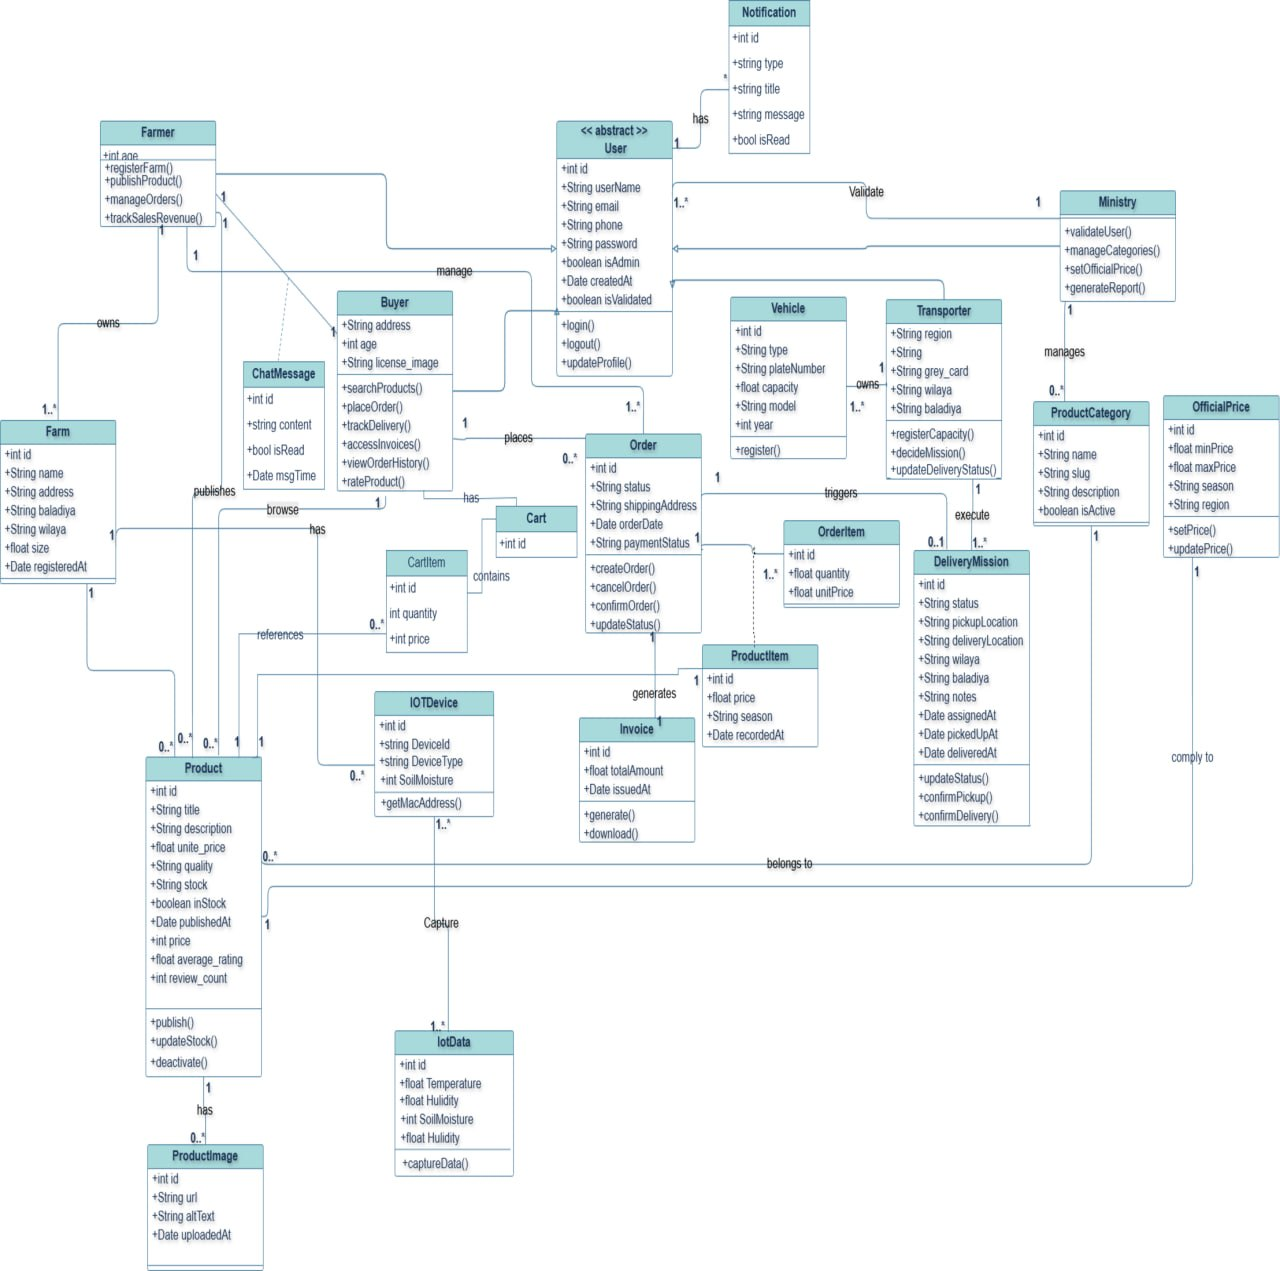
\includegraphics[height=0.84\textheight]{images/diagrammes/photo_2026-05-16_18-53-56}
		\caption{Class Diagram of the System}
	\end{figure}
